
\chapter{Predicting spatial curvature $\Omega_K$ in globally $CPT$-symmetric universes}\label{chapter:theory} % Force line breaks with \\

\chapterabstract{
    Boyle and Turok's $CPT$-symmetric universe model posits that the universe was symmetric at the Big Bang, addressing numerous problems in both cosmology and the Standard Model of particle physics. We extend this model by incorporating the symmetric conditions at the end of the Universe, which impose constraints on the allowed perturbation modes. These constrained modes conflict with the integer wave vectors required by the global spatial geometry in a closed universe. To resolve this conflict, only specific values of curvature are permissible, and in particular the curvature density is constrained to be $\Omega_K \in \{-0.016, -0.011, -0.004, \ldots\}$, consistent with \textit{Planck} observations.
}


\section{Introduction}

In this chapter, we investigate the impact of this periodic global structure on cosmological perturbations. Previous work by \citet{2022PhRvD.105h3514L} has explored this concept within the context of flat universes. They found that the physical solutions should not just symmetric at the Bang (satisfying Neumann IC), but also be symmetric or anti-symmetric at the future conformal boundary. The periodic conditions constrain the allowed wave vectors for perturbations to be some discrete values, which have observable effects on the Cosmic Microwave Background (CMB) power spectrum~\cite{2022PhRvD.105h3515B,2022PhRvD.105l3508P}.

Building on this work, we extend the analysis of \citet{2022PhRvD.105h3514L} to include curved universes. Our findings indicate that the discrete wave vectors imposed by the future conformal boundary conflict with the one from spatial boundary conditions in a closed universe. To reconcile this conflict, only specific values of curvature are permissible, which are consistent with the observations from \texttt{Planck 2018}~\cite{2020A&A...641A...6P}. 

\section{Background and perturbations} 
We build on the derivation presented in \citet{2022PhRvD.105h3514L} and extend it to a curved universe. The perturbed FLRW metric can be written as:
\begin{equation}
    ds^2 = a^2 \left[-(1 + 2\Phi)d\eta^2 + (1 - 2\Phi)\left(\frac{1}{1-\kappa r^2}dr^2+r^2d\Omega^2\right) \right],
\end{equation}
where \(\Phi\) is the perturbation in the Newtonian gauge, and $\kappa$ controls the spatial curvature of the universe.

We analyse the evolution of the background in conformal time \(\eta\) instead of physical time to render explicit the periodic behaviour of the universe. Following Lasenby~\cite{2022PhRvD.105h3514L}, only three components are considered: dark energy $\lambda$, radiation $r$, and spatial curvature $\kappa$, omitting matter. The zero-order Friedmann equations are: 
\begin{equation}\label{eq:friedmann_eq_theory}
    \dot{a}^2 = \tfrac{1}{3}\lambda a^4 - \kappa a^2  + \tfrac{1}{3} r, \qquad 
    \ddot{a} = \tfrac{2}{3}\lambda a^3 - \kappa a,
\end{equation}
where \(\hbar = c = 8\pi G = 1\) and dots denote \(d/d\eta\).

The solution to \cref{eq:friedmann_eq_theory} can be expressed as a Jacobi elliptic function~\cite{2021arXiv210906204B}, which exhibits periodic global structure in conformal time. The universe begins at the Big Bang \(a = 0\), evolves to the end of the universe at \(a=\infty\) at a finite conformal time \(\eta_{\infty}\) termed the future conformal boundary (FCB), and then returns from the future boundary back to a future Big Bang, starting the cycle over again. However, this cyclic behaviour does not by default hold for perturbations. To maintain the behaviour, the perturbations should be symmetric not just at the Bang, but also at the FCB. The symmetry constrains the allowed modes of perturbations (see \cref{fig:a_perturbations-eta}).
\begin{figure*}[!ht]\centering
     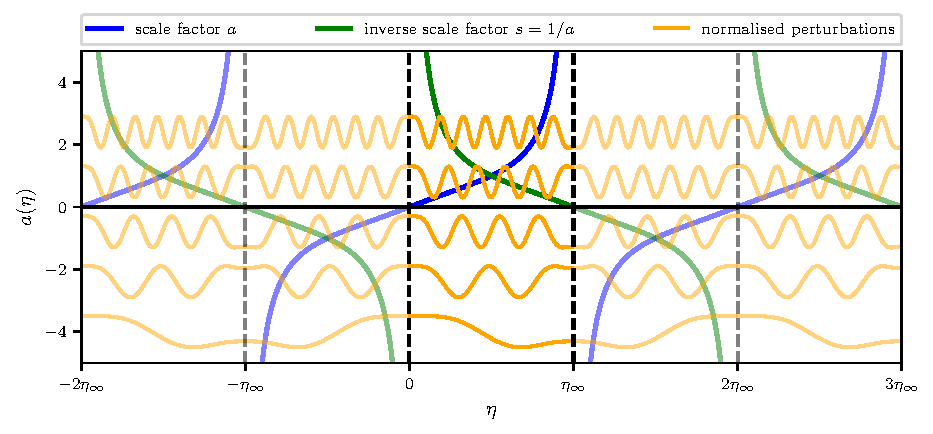
\includegraphics{./parts/part1/figures/a_perturbations-eta.pdf}
     \caption{Evolution of the scale factor \(a\), its reciprocal \(s\equiv 1/a\), and the first five allowed perturbations which are (anti)-symmetric about the future conformal boundary. The perturbations have been normalised to have constant oscillatory amplitude across cosmic time for clarity.}
     \label{fig:a_perturbations-eta}
\end{figure*}

To analyse the perturbations, we write the first-order Einstein equation as:
\begin{equation}\label{eq:perturbation_eq}
    \ddot{\Phi} + 4aH\dot{\Phi} + \tfrac{1}{3}(k^2 + 4a^2\lambda-12\kappa)\Phi = 0.
\end{equation}
where \(k\) is the comoving wave vector of the perturbation. Switching the independent variable from conformal time $\eta$ to scale factor $a$, one finds
\begin{equation}\label{eq:perturbation_a}
    (\lambda a^2 - 3\kappa + \frac{r}{a^2} )\Phi'' + (6\lambda a - \frac{15\kappa}{a} + \frac{4r}{a^3})\Phi' + (4\lambda+\frac{k^2-12\kappa}{a^2})\Phi = 0,
\end{equation}
where a prime denotes \(d/da\).

One degree of freedom between \(r\) and \(\lambda\) can be removed from \cref{eq:friedmann_eq_theory,eq:perturbation_a} by fixing the scaling of \(a\). Following~\cite{2022PhRvD.105h3514L}, \(r = \lambda\) is chosen, equivalent to demanding \(a=1\) when the energy density of matter radiation and dark energy are equal, after which \cref{eq:perturbation_a} becomes
\begin{equation}\label{eq:Phi_ODE}
    a(a^4 - 2a^2 \tilde\kappa + 1) \Phi'' + (6a^4- 10a^2 \tilde\kappa + 4 ) \Phi' + a(4a^2 + \tilde{k}^2-8\tilde\kappa) \Phi = 0, 
\end{equation}
\vspace{-2.5em}
\[ \text{where} \qquad
    \tilde{k} \equiv k/\sqrt{\lambda}, \qquad \tilde \kappa \equiv \frac{3}{2\lambda}\kappa\]
are the dimensionless wave vector and curvature respectively. The factor $\frac{3}{2}$ in $\tilde\kappa\equiv \frac{3}{2\lambda}\kappa$ is chosen such that $\tilde\kappa=1$ corresponds to the transition between a turnaround and a de-Sitter universe, which will be explained later. This equation reduces to eq.~(23) in~\citet{2022PhRvD.105h3514L} when \( \tilde\kappa = 0 \).
Note that if we replace \(\Phi(a)\) with \(\varphi(a) \equiv a^2 \Phi(a)\), the equation remains invariant under the transformation \({a\leftrightarrow1/a}\). This symmetry is important in the next section when considering perturbations passing through the FCB as \(a\rightarrow \infty\).

This equation can be solved analytically, yielding two solutions, both expressed in terms of Heun functions. Observing the CMB power spectrum told us that the solution must satisfy the Neumann initial conditions \(\Phi(a = 0) = C\) and \(\Phi'(a = 0) = 0\), where \(C\) is a constant \footnote{The conventional explanation is from cosmic inflation: the perturbation remains frozen at the beginning and starts oscillating after crossing the horizon \((k = aH)\); on the other hand, in CPT-symmetric universe model, the perturbation solutions should be symmetric at the Big Bang, which naturally satisfy Neumann IC}. Here are the two solutions:
\begin{equation}
\begin{aligned}\label{eq:Heun}
    \Phi_1(a) &= \text{HeunG} \left( -1+2\tilde\kappa \tilde a_+^2,\frac{\tilde k^2-8\tilde\kappa}{-4 \tilde a_-^2},\frac{1}{2},2, \frac{5}{2},\frac{1}{2},a^2\tilde a_+^2\right)\\
    \Phi_2(a) &= \text{HeunG}\left(-1+2\tilde\kappa \tilde a_+^2,\frac{\tilde k^2-2\tilde\kappa}{-4\tilde a_-^2},-1,\frac{1}{2},-\frac{1}{2},\frac{1}{2},a^2\tilde a_+^2\right)\\
    &\tilde a_{\pm}=\sqrt{\tilde\kappa\pm\sqrt{\tilde\kappa^2-1}}
\end{aligned}
\end{equation}
where \(C\) is chosen to be 1 without loss of generality. \(\tilde{a}_{\pm}\) are the extreme values of the scale factor, corresponding to \(\dot{a}=0\) in \cref{eq:friedmann_eq_theory}. Although both solutions meet these conditions, $\Phi_2$ exhibits increasing amplitude during oscillations and eventually diverges as \(a \to \infty\), rendering it non-physical. Therefore, we select the physical solution $\Phi_1$, which oscillates and decays as \(a \to \infty\).


\section{Constraints from the future conformal boundary}\label{sec:constrain_FCB}
Next, we investigate the behaviour of perturbations near the FCB.  For universes with curvature \( \tilde{\kappa} \equiv \frac{3}{2\lambda}\kappa > 1 \), the scale factor \(a\) reaches a maximum before they collapse in a ``big crunch'', which are not physically relevant, since we observe an accelerating Universe today. This implies that the Universe cannot possess excessive curvature, establishing an upper limit of \(\tilde{\kappa} < 1\). In this case, the scale factor \(a\) approaches infinity at the FCB.
Consequently, we should consider the reciprocal scale factor \( s \equiv 1/a \). Because of the symmetry in \cref{eq:Phi_ODE}, the solution can be expressed as \(\Phi(s)= s^4 \Phi(a(s)) \). As a result, the solution would continue oscillating through the FCB until the future Big Bang. \citet{2022PhRvD.105h3514L} found that most perturbations diverge before reaching the future Big Bang. Only those solutions that are finite and symmetric or antisymmetric at the FCB remain non-singular (see \cref{fig:a_perturbations-eta}). This symmetry requirement means that only a discrete spectrum of wavevectors are allowed.

To calculate the discrete spectrum of wave vectors, we re-write the perturbation solution into an integral form \cref{eq:integration_sol}, where the sine component captures the solution's oscillatory nature:
\begin{equation}\label{eq:integration_sol}
\begin{aligned}
    \Phi(a) &= \frac{3\sqrt{a^4 + (\tilde{k}^2 -2\tilde\kappa)a^2 + 1}}{a^3\tilde{k}\sqrt{(\tilde{k}^2 -2\tilde\kappa)^2 - 4}} \sin\theta(\tilde k,\tilde\kappa,a),\\
    \theta = \int_0^a &\frac{\tilde{k} a'^2 \sqrt{(\tilde{k}^2 -2\tilde\kappa)^2 - 4}}{\sqrt{1 + a'^4 - 2\tilde\kappa a'^2} \left( a'^4 + (\tilde{k}^2 -2\tilde\kappa)a'^2 + 1 \right)} da',
\end{aligned}
\end{equation}
The integration in \(\theta(a)\) can be expressed as an incomplete elliptic integral of the third kind \(\Pi\):
\begin{equation}\label{eq:psi_elliptic}
\begin{aligned}
    \theta(a) = \tilde{k} \tilde a_- \times \Bigg[ &\Pi\left( \frac{a}{\tilde a_-}, -\frac{1}{2}\tilde a_-^2 \tilde K_{-}^2, \tilde a_-^2 \right) \\
    - &\Pi\left( \frac{a}{\tilde a_-}, -\frac{1}{2}\tilde a_-^2 \tilde K_{+}^2, \tilde a_-^2 \right) \Bigg],\\
\end{aligned}
\end{equation}
\vspace{-1em}
\begin{equation*}
\begin{aligned}
    &\Pi(z,\nu,k)=\int_0^z \frac{1}{(1-\nu t^2)\sqrt{1-t^2}\sqrt{1-k^2t^2}} dt,\quad
    &\tilde K_{\pm}=\sqrt{(\tilde{k}^2 -2\tilde\kappa) \pm \sqrt{(\tilde{k}^2 -2\tilde\kappa)^2 - 4}}.
\end{aligned}
\end{equation*}
For the flat case (\(\tilde\kappa=0\)), the solution \cref{eq:integration_sol,eq:psi_elliptic} reduces to eq.~(26-28) in~\citet{2022PhRvD.105h3514L}.

If we require the solution to be (anti)symmetric at the FCB, the cycles of oscillation should be complete at the boundary. This implies that the angle \(\theta\) in the sine function should equal \( n\frac{\pi}{2} \) at \( a \rightarrow \infty \). 
\begin{equation}\label{eq:theta}
    \theta(\tilde{k}, \tilde\kappa, a \rightarrow \infty) \overset{!}{=} \frac{n\pi}{2}.
\end{equation}
The corresponding \(\tilde{k}\) are the allowed values of discrete wave vectors. The function \(\theta(\tilde k,a\rightarrow\infty)\) with different \(\tilde\kappa\) is illustrated in \cref{fig:theta_diffK}. While increasing the curvature value \(\tilde\kappa\), \(\theta\) becomes steeper, and the corresponding discrete wave vectors \(\tilde{k}\) have smaller spacing. 


\begin{figure}[htbp]
    \centering
    % Left Subfigure
    \begin{subfigure}[b]{0.51\textwidth}
        \centering
        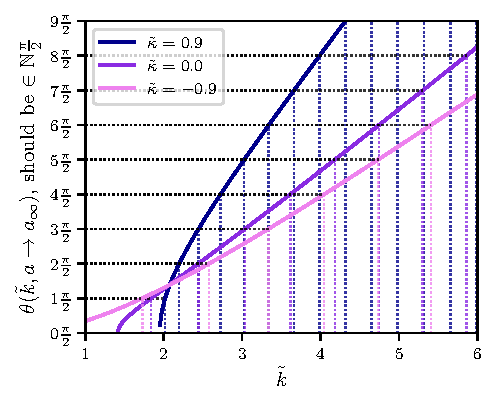
\includegraphics[width=\textwidth]{./parts/part1/figures/theta_discretek.pdf}
        \caption{Phase of perturbations \(\theta(\tilde{k},a\rightarrow \infty)\) with different curvature \(\tilde\kappa\). Larger \(\tilde\kappa\) results in a steeper curve. The value of \(\theta\) should be \(\frac{\pi}{2}n, n\in\mathbb{N}\), where the corresponding \(\tilde k\) are the allowed wave vectors forming a discrete spectrum.}
        \label{fig:theta_diffK}
    \end{subfigure}%
    \hfill
    % Right Subfigure
    \begin{subfigure}[b]{0.46\textwidth}
        \centering
        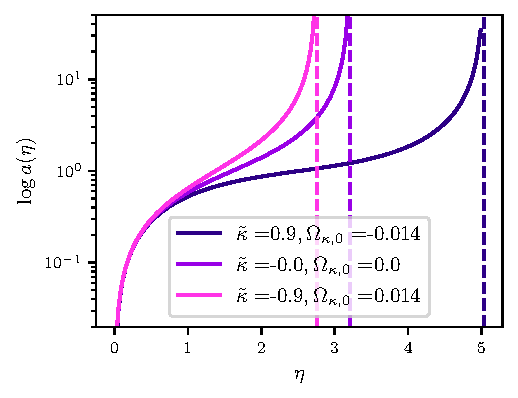
\includegraphics[width=\textwidth]{./parts/part1/figures/eta-log_a.pdf}
        \caption{Evolution of scale factor $a$ with different curvature. When curvature increasing ($\Omega_{\kappa,0}$ becomes more negative), it takes more time for $a$ to evolve to infinity. In other words, the age of the universe $\eta_\infty$ increase.}
        \label{fig:eta-log_a}
    \end{subfigure}
\end{figure}

The reason for this is that the slope of $\theta$ is proportional to the age of the universe $d\theta(a\rightarrow \infty)/d\tilde k=\eta_\infty /\sqrt{3}$. Taking standing waves in a finite tunnel for analogy, only discrete wave vectors are allowed $k=n\frac{\pi}{L}$, where the slope of phase $dn/dk=L/\pi$ is proportional to the length of the tunnel (analogous to the age of the universe in our case). And since the age of the universe increases when the curvature value increases (see \cref{fig:eta-log_a}), $\theta$ also becomes steeper.

\section{Implications for spatial curvature \(\Omega_K\)} 
These observations have significant implications for closed universes, where the compactness of spacial slices necessitates integer wave vectors (Sec.~2.4 in~\cite{2017CCoPh..22..852T}). This requirement is generally in conflict with the discrete spectrum of wave vectors arising from FCB considerations, prompting the question of whether this conflict can be resolved by matching the two discrete sets.

In \cref{fig:theta_diffK} \(\theta(\tilde{k})\) approaches a straight line for high-\(k\) modes due to perturbations oscillating as \(\sim \cos(\tilde{k}\eta/\sqrt{3})\).
This implies that the allowed wave vectors are equally spaced for high-\(k\) modes. By adjusting \(\tilde{\kappa}\), we can align the allowed wave vectors to be integers. 
Note that this method does not work for low-\(k\) modes, as \(\theta(\tilde{k})\) cannot be approximated as a straight line. In these cases, the perturbation solution, which is periodic in both spatial and temporal coordinates, must be expressed as a specific linear combination of the two discrete sets (details will be explained in \cref{chapter:low-k}). As \(k\) increases, the mode corresponding to \(n \sim k\) becomes increasingly dominant, and eventually, the two sets align in the high-\(k\) regime. This is the subject of current investigation.

Also, keep in mind that the unit of \(\tilde{k}\) differs from that of the integer wave vectors \(k_{\text{int}}\). The transformation between them can be expressed as: \(\tilde{k}\equiv  \sqrt{\frac{2\tilde{\kappa}}{3}} \sqrt{k_{\text{int}}(k_{\text{int}}+2) }  \approx \sqrt{\frac{2\tilde{\kappa}}{3}} k_{\text{int}}\) in high-\(k\) modes. Consequently, the actual gradient is given by:
\begin{equation}
\frac{d\theta}{dk_{\text{int}}}(\tilde{\kappa},\tilde{k}\gg 1,a\rightarrow \infty) \approx \sqrt{\frac{2\tilde{\kappa}}{3}}\frac{\eta_{\infty}(\tilde{\kappa})}{\sqrt{3}} \overset{!}{=} N^{\pm 1}\frac{\pi}{2},
\end{equation}
where to match the integer wave vectors, the gradient should be \(N\frac{\pi}{2}\) or \(\frac{1}{N}\frac{\pi}{2}\) (where \(N\in\mathbb{N}\)), corresponding to either sparser discrete \(\theta\) or sparser \(k_{\text{int}}\) (see \cref{fig:theta_kint}). Since the gradient depends on \(\tilde{\kappa}\), this constrains the allowed curvature values. Some allowed \(\tilde{\kappa}\) values are shown in \cref{fig:Slope_kc}. The gradient increases with \(\tilde{\kappa}\) and approaches infinity as \(\tilde{\kappa}\) approaches unity, the maximum allowed curvature value. Beyond this value, the universe would collapse, resulting in a crunch. 

% As for the minimum, while all rational values of \(R\) are technically allowed, values with larger denominators \(B\) are less favoured by CMB observations. This is because larger \(B\) corresponds to wider spacing between discrete \(k_{\text{int}}\) values, which contradicts the CMB data, where most \(k_{\text{int}} \in \mathbb{N}\) are permitted. Therefore, values of \(\tilde{\kappa} < 0.672\) (where \(R = 1\)) are less preferred.


\begin{figure}
     \centering
        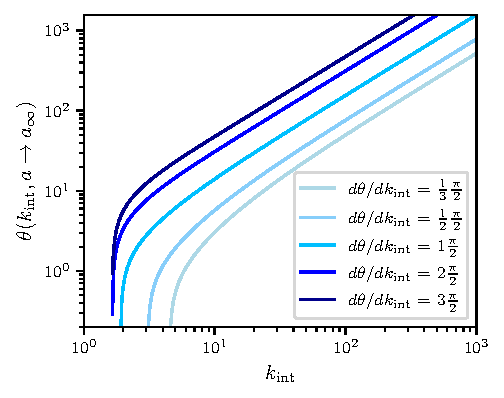
\includegraphics[width=0.6\textwidth]{./parts/part1/figures/theta-kint_loglog.pdf}
        \caption{Phase of perturbations $\theta$, in log-log plot. In the high-\(k\) mode, the gradient of \(\theta\) approximates a straight line, indicating that the discrete wave vectors are equally spaced. In a closed universe, these wave vectors must be integers, constraining the gradient $d\theta/dk_{\text{int}}$ to be \(N\frac{\pi}{2}\) or \(\frac{1}{N}\frac{\pi}{2}\) (where \(N\in\mathbb{N}\)). Lines with gradient \(= \left[\frac{1}{3}\frac{\pi}{2}, \frac{1}{2}\frac{\pi}{2}, 1\frac{\pi}{2}, 2\frac{\pi}{2}, 3\frac{\pi}{2}\right]\) are plotted, corresponding to \(\tilde{\kappa} = [0.113, 0.238, 0.672, 0.986, 0.999]\).}
        \label{fig:theta_kint}
\end{figure}

\begin{figure}
     \centering
        
\includegraphics[width=0.7\textwidth]{./parts/part1/figures/slope_kappa.pdf}
        \caption{The gradient of the phase of perturbations \(\theta\), as a function of \(\tilde\kappa\). The gradient constraint determines the preferred curvature values.}
        \label{fig:Slope_kc}
\end{figure}

The predicted values of \(\tilde{\kappa}\) are then transformed to the current curvature density \(\Omega_K=-2\tilde{\kappa}\sqrt{\Omega_\Lambda\Omega_r}\) and compared with the \texttt{Planck 2018} data (\cref{fig:Planck_kappa}). 
The \(\tilde{\kappa}\), for unit gradient, corresponds to \(\Omega_K\sim -0.011\). The maximum curvature, \(\tilde{\kappa}=1\), corresponds to \(\Omega_K\sim -0.016\). Although this is closer to flat than the observational value of \(-0.044^{+0.018}_{-0.015}\)~\cite{2021PhRvD.103d1301H,2020NatAs...4..196D,2020A&A...641A...6P}, incorporating matter into our model would likely yield more precise predictions. Despite its simplicity, our model recovers curvature values consistent with observational data.

\begin{figure}
     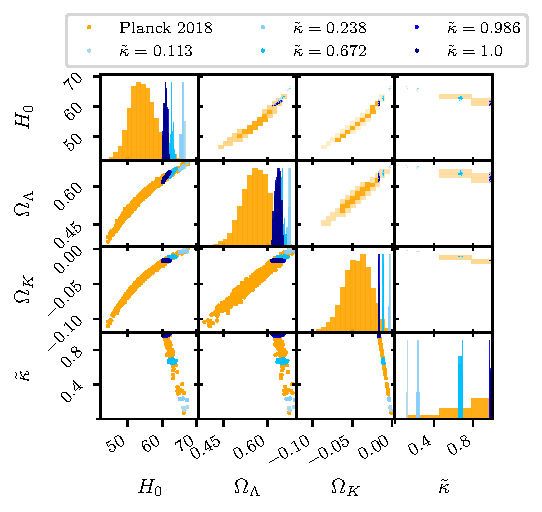
\includegraphics[width=0.9\textwidth]{./parts/part1/figures/Planck_kappa.pdf}
     \centering
     \caption{Comparison of predicted curvature values with \texttt{Planck 2018} data (\texttt{base\_omegak\_plikHM\_TTTEEE\_lowl\_lowE} from~\cite{2020A&A...641A...6P}). Predicted curvature values from \cref{fig:Slope_kc} are shown.}
     \label{fig:Planck_kappa}
\end{figure}


\section{Conclusion} 
In this chapter, we extended the work of \citet{2022PhRvD.105h3514L} and \citet{2021arXiv210906204B} by solving the first-order perturbation equation to derive analytic solutions. These solutions remain physical if they exhibit symmetry or antisymmetry at the FCB. This temporal boundary condition imposes a discrete spectrum on the wave vectors, which conflicts with the integer wave vectors derived from the spatial compactness of closed universes. Since both sets of discrete \(k\) values exhibit equal spacing in the high \(k\) regime, we can reconcile them by constraining the spatial curvature to specific values. 

To refine the predictions of this allowed curvature spectrum further, we need to solve the perturbations numerically in a more detailed universe model that includes matter and radiation anisotropy. The resulting solutions will be used to generate the CMB power spectra, which will then be compared with observational data, following the methodologies of~\cite{2022PhRvD.105h3515B} and~\cite{2022PhRvD.105l3508P}. These will be explain in the next chapter. 


% \vfill
% \pagebreak

% \appendix

% \section{Perturbation solution in Heun function form}

% \begin{equation}
% \begin{aligned}
%     &\Phi(a) = 
%     \left(1 + 2(1 - 2 \tilde\kappa^2) a^4 + a^8\right)^{1/8} \left(\frac{i a^2}{\alpha} - 1\right)^{-\gamma} (i \alpha a^2 + 1)^{\gamma} \\
%     &\times \exp\left(-\frac{1}{4}\tanh^{-1}\left(\frac{2a^2\tilde\kappa}{1+a^4}\right)+\frac{i +\tilde\kappa}{2\sqrt{\tilde\kappa^2-1}} \tanh^{-1} \left(\frac{-a^2+\tilde\kappa}{\sqrt{\tilde\kappa^2-1}}\right) \right)\\
%     &\times \text{HeunG}\left(-\frac{1}{\alpha^2}, -\frac{i \tilde{k}^2-i8\tilde\kappa - 5 \alpha}{4 \alpha}, 1, \frac{5}{2}, \frac{5}{2}, \frac{1}{2}, \frac{i a^2}{\alpha}\right),
% \end{aligned}
% \end{equation}


% where \(\alpha\) and \(\gamma\) are given by:
% \begin{equation*}
%     \alpha = i \tilde\kappa + \sqrt{1 - \tilde\kappa^2}, \quad \gamma = \frac{\alpha(\alpha - 1)}{2 \alpha^2 + 2}.
% \end{equation*}

\printbibliography[heading=subbibintoc, title={References for Chapter \thechapter}]
% ****** End of file ******
